\documentclass[preprint, 12pt]{elsarticle}

%% Use the option review to obtain double line spacing
%% \documentclass[preprint,review,12pt]{elsarticle}

%% Use the options 1p,twocolumn; 3p; 3p,twocolumn; 5p; or 5p,twocolumn
%% for a journal layout:
%% \documentclass[final,1p,times]{elsarticle}
%% \documentclass[final,1p,times,twocolumn]{elsarticle}
%% \documentclass[final,3p,times]{elsarticle}
%% \documentclass[final,3p,times,twocolumn]{elsarticle}
%% \documentclass[final,5p,times]{elsarticle}
%% \documentclass[final,5p,times,twocolumn]{elsarticle}

\usepackage{graphicx}
\usepackage{subcaption}
\usepackage{amssymb}
\usepackage{siunitx}
\usepackage{lipsum}
\usepackage[]{color}
\usepackage{lineno}
\usepackage[]{hyperref}
%
\DeclareSIUnit{\Wsqcm}{\watt\per\square\centi\meter}
%
\journal{Journal Name}

\begin{document}

\begin{frontmatter}

%% Title, authors and addresses

%\title{Particle--in--cell simulation of the dynamics of short--pulse laser
%irradiated multilayer targets and x--ray reflectometry diagnostics.}

\title{Particle--in--cell simulations of grazing-incidence x-ray scattering of
surfaces upon high--intensity laser irradiation}


%% use the tnoteref command within \title for footnotes;
%% use the tnotetext command for the associated footnote;
%% use the fnref command within \author or \address for footnotes;
%% use the fntext command for the associated footnote;
%% use the corref command within \author for corresponding author footnotes;
%% use the cortext command for the associated footnote;
%% use the ead command for the email address,
%% and the form \ead[url] for the home page:
%%
%% \title{Title\tnoteref{label1}}
%% \tnotetext[label1]{}
%% \author{Name\corref{cor1}\fnref{label2}}
%% \ead{email address}
%% \ead[url]{home page}
%% \fntext[label2]{}
%% \cortext[cor1]{}
%% \address{Address\fnref{label3}}
%% \fntext[label3]{}


%% use optional labels to link authors explicitly to addresses:
%% \author[label1,label2]{<author name>}
%% \address[label1]{<address>}
%% \address[label2]{<address>}

\author[1]{M. Banjafar}
\author[2]{L. Randolph}
\author[3]{T. Kluge}
\author[3]{M. Bussmann}
\author[1]{A .P. Mancuso}
\author[3]{T. E. Cowan}
\author[1]{C. Fortmann-Grote}
\author[2]{C. Gutt}
\author[1]{M. Nakatsutsumi}
%
\address[1]{European XFEL GmbH, Holzkoppel 4, 22869 Schenefeld, Germany}
\address[2]{Department of Physics, University of Siegen, D-57072 Siegen, Germany}
\address[3]{Helmholtz-Zentrum Dresden-Rossendorf, Bautzner Landstraße 400, 01328 Dresden, Germany}

% Abstract
\begin{abstract}
  Interaction of solid materials with laser pulses
  produces warm dense matter under controlled laboratory conditions.
  Multilayer targets of alternating high and low Z material layers of a few
  nanometer thickness open the possibility
  to study the laser--matter interaction dynamics as a volumetric effect by
  observing the multilayer Bragg peak in x--ray reflectometry experiments.
  We apply particle--in--cell simulations of
  the laser--target interaction and subsequent calculations of
  the reflectivity and diffuse x--ray scattering as a
  function of reflection angle and various time delays between the optical pump
  and the x--ray probe pulse delivered by an x--ray free--electron laser.
  We demonstrate that the combined measurement of reflectivity and
  diffuse scattering provides valuable information about the evolution of
  electron density gradients, temperature and ionization as a function of target
  depth and pump--probe time delay and Bragg peak position. Manifest limitations
  of the particle--in--cell method in the warm--dense--matter regime are
  demonstrated and discussed.
\end{abstract}
%
\begin{keyword}
Short pulse laser--matter interaction \sep particle--in--cell simulations \sep x--ray
diagnostics \sep x--ray free--electron laser
%% MSC codes here, in the form: \MSC code \sep code
%% or \MSC[2008] code \sep code (2000 is the default)
\end{keyword}
\end{frontmatter}
%
% Comment to suppress linenumbering.
\linenumbers
\begin{verbatim}
Thomas:
  * Experimental description should focus on giving the physical
  motivation of why we want to do surface diffraction at all
  * Simulation part should focus on showing
    (1) the qualitative plasma physics we expect
    (2) the differences between codes with respect to
      (a) different physics included (e.g. comparing with and without
      ionization, with and withou collisions etc)
      (b) different models, e.g.
        i) TF vs. Direct impact ionization
        ii) large collision frequency vs. low collision frequency
        iii) comparing a constant Coulomb logarithm vs. a T-dependent one
        iV) hydro vs. PIC
      (c) different model implementations (e.g. TF and ADK are different
      in PICLS and PIConGPU)
    (3) lay the foundation in showing what plasma physics is important and
    what the uncertainties in the numerical modeling are, so that in the
    scattering part one can focus on showing how to measure the physics
    and validate the codes
  * The scattering part has to derive much more stringent the connection
  between the measured quantities (e.g. beta, change of max(Q) position,
  fourier transform/rings) and plasma physical quantities (e.g. what
  exactly are slow/fast dynamics and how do they imprint on the speckle
  contrast? surface ripple correlation changes - where do they come from
  (should be explained in the sim-part) and how do the show up in the
  signal, what exactly expands and how/why does it imprint on the signal,
  what is the plasma physics measured by the ring-analysis?...)
\end{verbatim}
%
%%%%%%%%%%%%%%%%%%%%%%%%%%%%%
\section{Introduction\label{sec:Introduction}}%
High--intensity laser--matter interaction has a broad range of
applications such as laser driven fusion \cite{Lindl2004,Atzeni2004} laboratory
astrophysics \cite{Nettelmann2008a}, proton acceleration \cite{Pukhov2001},
high--harmonic generation \cite{Chin2001,Ghimire2010}, and plasma mirrors
\cite{Kapteyn1991}.
Laser--matter coupling is largely dominated by the instantaneous electron density.
Substantial ionization due to \ldots can already be observed at
non--relativistic laser intensities (\SI{\ll
e18}{\Wsqcm}). A femtosecond optical laser pulse at moderate intensities
(\SIrange{e14}{e16}{\Wsqcm}) impinging on a thin
metal foil with a few tens of \si{\nm} thickness produces pressures in excess of
\SI{1}{\mega\bar}. Under such conditions, warm dense matter (WDM)
\cite{Lee2003a} forms with electron densities close to solid density and temperatures of a few
thousand to a few ten thousand \si{\K}. Due to its relevance in basic research
and technological applications, where WDM is often encountered as a transient
state, e.g. during the compression phase of laser driven fusion targets, there
is considerable interest in understanding the structure and dynamics of WDM.

Investigations of WDM are particularly challenging both from the experimental and from the
theoretical perspective. Extremely short pulsed particle sources are required to
probe the transient dynamics of WDM, with typical time scales ranging from a
few \si{\fs} (electron-electron collision rates) to the \si{\ps} regime
(electron--ion equilibration, hydrodynamic relaxation). Recently, laser--plasma driven x--ray sources
and free--electron lasers have become the state--of--the--art sources for this
research \cite{Lee2003}, owing to the high penetrability of x--rays in solid
density targets as compared to optical probes. These two features: short pulses,
an short wavelengths allow to apply inelastic scattering and
spectroscopic techniques such as x--ray Thomson scattering \cite{Glenzer2009}
and x--ray absoption spectroscopy \cite{Torchio2016} to infer volumetric
information from WDM targets.

The interpretation and analysis of experimental data
rely on theoretical models
and numerical simulations which have their own difficulties.
This is mainly due to WDM being located in a peculiar region of the density--temperature phase
diagram with temperatures comparable to both the electrons' Fermi energy and the
potential energy. These conditions give rise to partial quantum degeneracy and
moderate coupling. On top, the electron and ion subsystems often have quite distinct
temperatures and densities, requiring different theoretical approaches to treat
either one.

Technological applications such as high--harmonic generation and particle
acceleration operate with relativistic intensities in excess of
\SI{e18}{\Wsqcm}. Prepulse contrast ratios of  \numrange{e-4}{e-5}, which, based
on today's standards, are considered low, effectively mean that the main pulse
interacts not with the cold, unperturbed target but rather with warm dense
matter. Plasma mirrors take advantage of precisely this effect. The prepulse
makes the mirror surface reflective for the main pulse and thereby improves the
temporal contrast. It is hence of paramount interest to resolve the structure
and dynamics of the interface between a driven WDM target and the vacuum.

In this work, we demonstrate the applicability of x--ray reflectometry (XRR) and
grazing indicence x--ray diffraction (GIXRD) with multilayered targets
to simultaneously probe the target's surface and volumetric response to the
exitation by moderate intensity optical laser pulses.
We apply particle--in--cell simulations to model the
laser--matter interaction of a moderate intensity \si{\fs} laser pulse with
the multilayer target. From the simulated electron density distribution we then
calculate the reflectivity and diffuse scattering via the dielectric function.
We find that the multilayer reflectivity at the Bragg angle decreases
substantially as the incoupled laser energy propagates through the target and
radiation damage processes deteriorate the sharpness of multilayer interfaces
and periodicity. We show how to identify various processes during and after the
interaction with the optical laser pulse in the reflectivity signal and the
diffuse scattering.

It should be emphasized that our results must be treated
with care since the WDM regime is certainly at or beyond the limits of validity
for this technique. In fact, quantitative modeling of WDM is a critical challenge for kinetic method such as
particle--in--cell mainly due to (a) difficulties
in describing the ionization dynamics; (b) uncertainty about electron--ion
collision frequency in this non--Spitzer \cite{Spitzer1953} regime, which governs absorption, heat transfer and plasma
conductivity; and (c) violation of the heat conduction models laser excited
plasmas with steep temperature gradients.
Depending on the model and implementation,
atomic physics, ionization dynamics, and collisions are either missing or
treated within an ad-hoc model. Our results can therefore only give a
qualitative estimate of the experimental observables.
It is with these caveats in mind that for each
condition, we performed multiple PIC simulation runs with different models for
ionization and collisions as well as different spatial resolutions (grid size).

The paper is organized as follows:
Section~\ref{sec:Experiment} describes the experimental geometry underlying our
simulations. We briefly outlne the theoretical background in
Section~\ref{sec:Theory}, while
Section~\ref{sec:Results} contains the simulation results
from the PIC runs and the optical response calculations. The final
Section~\ref{sec:Discussion} discusses our results for the experimental
observables and, in particular,
the observed inconsistencies between different PIC runs and how these can be
linked to shortcomings of the PIC method.

%The periodicity in the
%direction normal to the target surface, with period $D$ gives rise to a pronounced resonance in
%the reflectivity as function of incidence angle, i.e. when the transfer
%wavevector $k\left|\vec k_{f}-\vec k_{i}\\right| = 2\pi / D$. By observing this
%multilayer Bragg at different time delays between the optical laser pump pulse
%and the x--ray probe, we can monitor the propagation of the incoupled laser
%energy through the volume.
%
%%%%%%%%%%%%%%%%%%%%%%%%%%%%%
\section{Experimental configuration\label{sec:Experiment}}
\begin{verbatim}
TBD: Motoaki
\end{verbatim}
%
\begin{figure}[ht]
  \begin{center}
    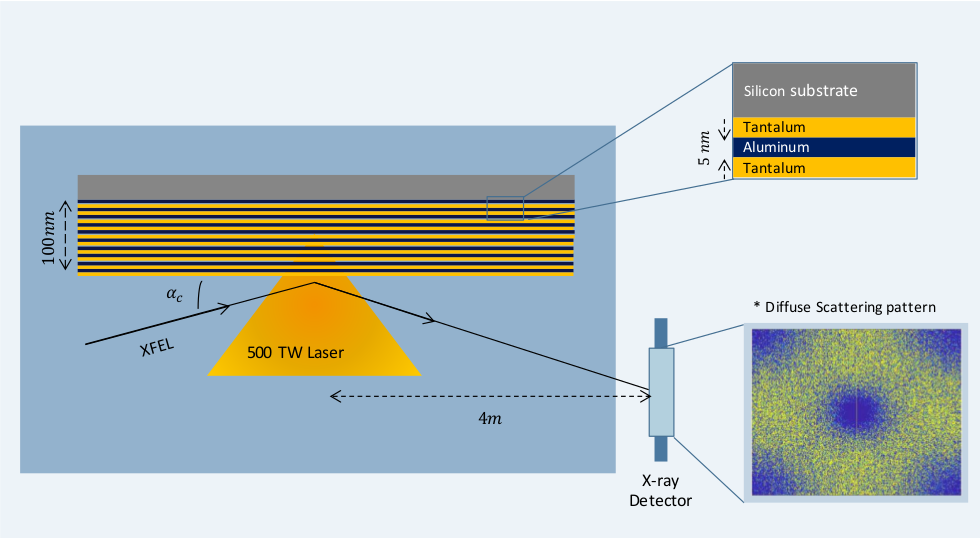
\includegraphics[width=0.8\textwidth,angle=0,clip]{figures/experiment_setup.png}
  \end{center}
  \caption{Experimental configuration for combined x--ray diffraction and
    grazing--incidence x--ray scattering measurements of laser--matter
    interaction. A short pulse \SI{800}{\nm} pulse drives creates warm dense
    matter on the target surface. The system is subsequently probed by an x--ray
    free--electron laser pulse under a shallow angle of incidence. Specular and
    diffuse scattering are observed in a 2D x--ray detector.
  }
  \label{fig:experiment_setup}
\end{figure}
%
An optical laser pulse with plane wave profilde, \SI{800}{\nm} wavelength, and intensity $I =
\SI{1e16}{\Wsqcm}$ corresponds to $a_{0} = 0.068$. The pulse duration (full
width at half maximum) is $\tau_\text{FWHM}=\SI{50}{\fs}$, and focal spot size of 5 $\mu m$  comes
alongside the $y$ axis and incidents normally on the front of multilayer (ML)
target, which is a 10 times reps of Tantalum, $n_{Ta} = 5.55 \times 10^{22}$
$cm^{-3}$, and Aluminum ,$n_{Al} = 6.022 \times 10^{22}$ $cm^{-3}$,
double-layers. The thickness of each layer is 5 $nm$ and regarding the 20 $nm$
Silicon substrate,
The total thickness of the target is \SI{120}{\nm}.
%
%%%%%%%%%%%%%%%%%%%%%%%%%%%%%
\section{Modeling\label{sec:Theory}}
\subsection{The particle--in--cell method\label{sec:PIC}}
The 2D simulations were performed with PIConGPU \cite{Bussmann2013}
\marginpar{What about PICLS?}. A
schematic of the simulated target is shown in Fig.~\ref{fig:simulation_setup}.
The 2D simulation box of \SI{\approx 1}{\square\micro\meter} is divided into $4096 \times 4096$ cells with
\SI{2.5}{\angstrom} lateral cell
dimension.  The simulation time step is ${\Delta}t=\SI{5.89e-4}{\fs}$
and the total simulated time is \SI{527}{\fs} and covers the entire pulse
duration plus the expansion phase when the pulse has already left the target.
Three ionization models are applied: barrier suppression ionization (BSI)
\cite{TBD}, Thomas-Fermi (TF) \cite{TBD}, and tunnel ionization according to the ADK model \cite{TBD}.
%
\begin{figure}[ht]
  \centering%
  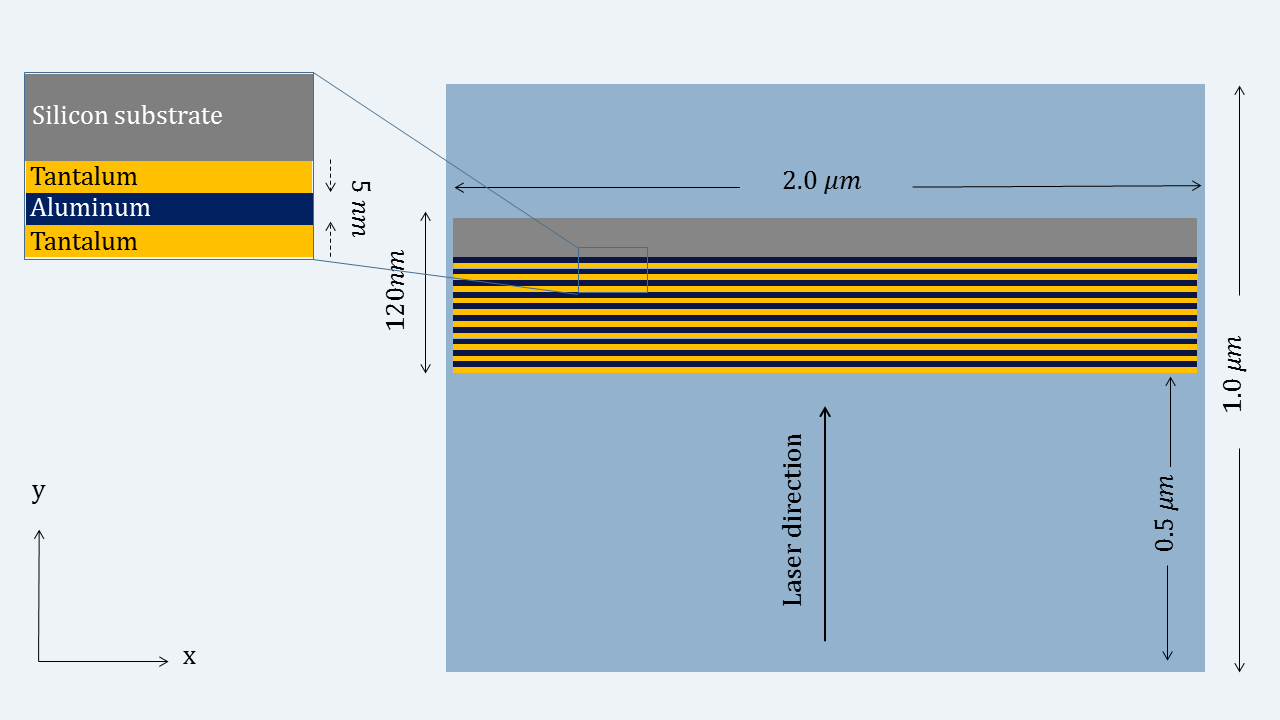
\includegraphics[width=0.8\linewidth]{figures/P_2.png}
  \caption{Sketch of the simulated target with laser and probe directions, layer
    thickness and overall dimensions.}
  \label{fig:simulation_setup}
\end{figure}
%
%%%%%%%%%%%%%%%%%%%%%%%%%%%%%
\subsection{The x--ray optical response: Specular reflectivity and diffuse scattering\label{sec:response}}
%
\begin{verbatim}
TBD: Lisa, Christian
\end{verbatim}
%
\lipsum[1]
%
%%%%%%%%%%%%%%%%%%%%%%%%%%%%%
\section{Results\label{sec:Results}}
\subsection{Electron densities from PIC\label{sec:electron_densities}}
Figure~\ref{fig:pic_edens_2D} shows the particle densities for free electrons
(first row), bound electrons (second row), and the total electron density (third
row) color coded as a function of transverse dimension ($x$) and longitudinal
($y$). Snapshots are taken at \SIlist{0;75;226;410}{\fs} of the simulation
$t=0$ corresponds to the moment when the peak of the laser pulse strikes the
target's surface. No substantial ionization was found for times $t<0$.
At $t=\SI{75}{\fs}$, the pulse has left the rear surface.
As the laser propagates through the target, it ionizes the target atoms both in
the low Z and high Z material of the multilayer structure. The bottom row shows
how the initially sharp interfaces between both materials wash out and how the
density contrast deteriorates. Globally, the periodicity of the structure
remains intact over the course of the simulated time.
The laser pulse is not able to penetrate more than a few nanometer (skin depth)
into the target and it is partially reflected when it reaches the critical density.
Due to the ponderomotive force, electrons at the front of target will be pushed
into the deeper layers. At present conditions of high electron densities
compared to the laser's critical density ($n/n_\text{cr} = \frac{}{}\simeq
\num{1e2}$), and moderate laser intensity, the  $\vec{J} \times \vec{B}$ term is
negligible compared to the dc-ponderomotive force \cite{TBD}.
However the magnetic part of the Lorentz force is able to pull some electrons out into the vacuum
thus maintaining zero field inside the target \cite{TBD}.
Most of these dragged electrons are pushed back into the target when the laser
field is reversed in the second half of the laser cycle, causing an oscillatory
movement in the target's surface normal direction.
%
\begin{figure}[ht]
  \centering
\includegraphics[width=1.0\linewidth]{figures/paper_plot.png}
  \caption{2D electron density maps}
  \label{fig:pic_edens_2D}
\end{figure}
%
Figure~\ref{fig:edens_1D} shows the total electron density averaged over the
transverse coordinate as a function of target depth.
During the laser pulse, the radiation pressure
suppresses expansion from the surface into the vacuum. The multilayer
target maintains its structure without significant change. After the laser pulse
($t\geq \SI{75.4}{\fs}$) we find expansion by a few nanometer. In absence of the
laser pulse, expansion accelerates and the surface rapidly expands up to \SI{20}{\nm} at
\SI{226}{\fs} and then at lower speed to \SI{40}{\nm} at \SI{452}{\fs}.
At these later times, the multilayer structure has also deteriorated but the
periodicity remains globally intact.
%
\begin{figure}[ht]
  \centering%
  
\includegraphics[width=0.8\linewidth]{figures/Paper_plot_1D.png}
  \caption{1D total electron density maps}
  \label{fig:edens_1D}
\end{figure}
%
\subsection{Collisions\label{sec:collisions}}
\begin{figure}[ht]
  \begin{center}
    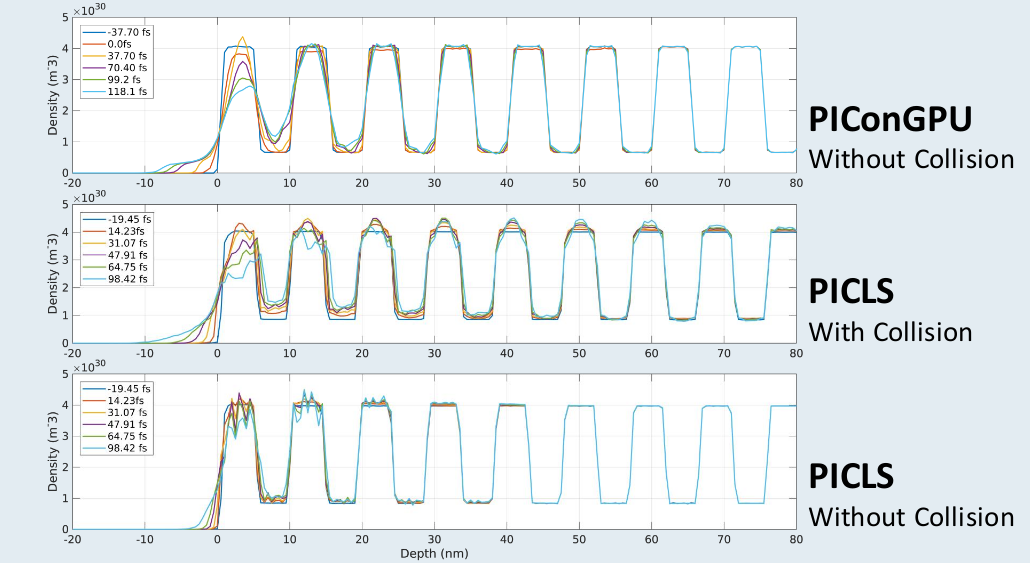
\includegraphics[width=.8\textwidth,angle=0,clip]{figures/ne_profiles_picongpu_vs_picls_collisions}
  \end{center}
  \caption{Electron density profiles from PIConGPU (top), without collisions,
    from PICLS  with (middle) and without (bottom) electron--ion collisions
    taken into account. Note that the PICLS results including collisions is
    closer to the PIConGPU result without collisions than the non--collisional
    PICLS simulation.
  }
  \label{fig:ne_collisions_pic}
\end{figure}
%
\subsection{Reflectivity\label{sec:reflectivity}}
\begin{verbatim}
TBD: Lisa, Christian
\end{verbatim}
%
\begin{figure}[ht]
  \begin{center}
    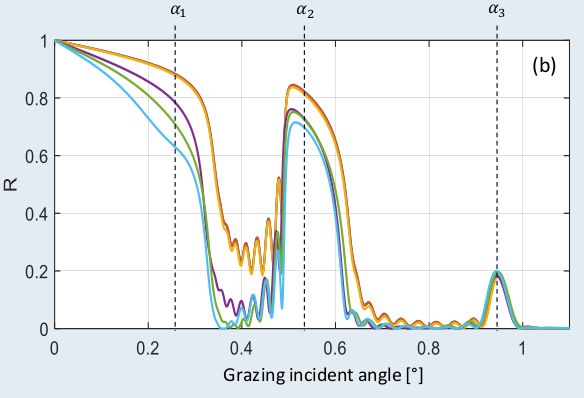
\includegraphics[width=.8\textwidth,angle=0,clip]{figures/TaAl_reflectivity}
  \end{center}
  \caption{Multilayer target reflectivity $R$ as function of angle of incidence
    and for different time delays after the peak of the optical pump laser has hit
    the target.
  }
  \label{fig:TaAl_reflectivity}
\end{figure}
%
\lipsum[2]
%
\subsection{Diffraction\label{diffraction}}
\begin{verbatim}
We need figures here
\end{verbatim}
%
\begin{figure}[ht]
  \begin{center}
    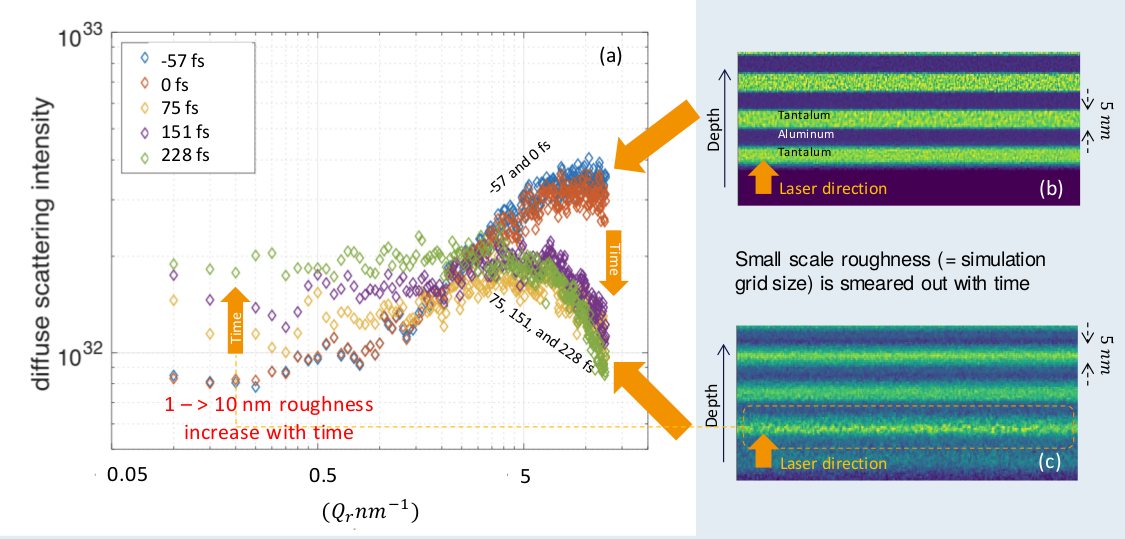
\includegraphics[width=.8\textwidth,angle=0,clip]{figures/TaAl_diffuse_scattering}
  \end{center}
  \caption{Diffuse scattering speckle contrast as function of time delay between
    optical pump laser and x--ray probe pulse.}
  \label{fig:TaAl_diffuse_scattering}
\end{figure}
{\color{blue}
%
Fig.~\ref{fig:diffuse_scatterin}
which displays three diffraction pattern as a function of $Q$ in x and y
direction in ln-scale corresponding to -51.8, 160.3, and 341.9 fs. The
diffraction images show the specular signal as a high intensive streak and also
the diffuse scattering signal as a ring around the center by which we are able
to interpret the scale of the roughness. That means larger ring for diffuse
scattering signal corresponds to the smaller scale roughness and vice versa. By
this definition, we can relate the large ring at -51.8 fs to the angstrom scale
roughness which are mainly due to random distribution of particles inside the
angstrom scale simulation cells. By the time the ring gets smaller and for
larger $Q$-values there is only a weak scattering signal that means the scale of
the roughness gets lager due to the irradiation. This dynamic can also be seen
in figure (radial intensity figure a) shows a more detailed distribution of the
radial intensity of scattered X-ray as a function of $Q$ for different time from
-70 fs (red) to 395.9 fs (blue). Figure (radial intensity figure a) depicts the
maximum of the scattered intensity as a function of time displaying a reduction
of intensity until its minimum value at 124.6 fs that correspond to the three
quarter of optical laser pulse.
To have a better image of these dynamics we considered some $Q$-rings with the
width of $\Delta Q \approx 0.08$ $nm^{-1}$ and different radius from 0.54 to
7.60 $nm^{-1}$ which are centered at the center of diffraction pattern ring as
it has been shown in figure (figure 5a of Lisa). The radius difference between
the rings is $\Delta Q_r \approx 0.08$ $nm^{-1}$. Figure (5b from Lisa) shows
the variation of the contrast $\beta$ for the smaller $Q$-rings up to radius
3.06 $nm^{-1}$ and figure (5c from Lisa) shows larger $Q$-rings. For the smaller
$Q$-rings which correspond to lagers scale roughness we see just a small
variation of contrast $\beta$. For instance, for 0.54 and 1.04 $nm^{-1}$,
corresponds to (length scale! ask Lisa) $nm$ in real space, one can just see
some fluctuations for $\beta$ by the time that means in large scale we are not
significant dynamics. But as we go to the larger $Q$-ring values there is an
obvious reduction of $\beta$ and faster dynamics for smaller scale roughness.

The electron dynamics found in the PIC data is directly mapped to observable
signatures in the x--ray diffraction pattens. Fig.~\ref{fig:XX}
shows the speckle contrast $\beta$ as a function time \marginpar{Right?}.
Higher values of $\beta$ correspond to slower dynamics.
Then, $\beta$ curve drops down rapidly that corresponds to
smaller intensity fluctuations and faster dynamics until 226 fs, from then it
the dynamics get faster with a slower speed. It is also shown in figure (Q as
time figure) that displays the variation of the Q-value as a function of time
for the maximum scattered X-ray intensity. Similar to the figure (contrast
figure), at 75.4 fs, right after the optical laser pulse, the Q-value drops down
to the 0.5 $nm^{-1}$ which means the scale of the roughness get larger during
this time. One can interpret the speed of the expansion from the slope of this
graph. For instance, from 75.4 to 200 fs, Q changes by 2 $nm^{-1}$ that
corresponds $\approx 1.5$ $nm$ in real space. Thus, the speed of the plasma
expansion during this time is about $10^{4}$ $m/s$.
}
%
%%%%%%%%%%%%%%%%%%%%
\section{Discussion\label{sec:Discussion}}
\begin{verbatim}
TBD: All
\end{verbatim}
%
\lipsum[3]
%%%%%%%%%%%%%%%%%%%%%%%%%%%%%
\section{Summary and Outlook\label{sec:summary}}
\begin{verbatim}
TBD: All
\end{verbatim}
%
\lipsum[4]
%%%%%%%%%%%%%%%%%%%%%%%%
\section*{Acknowledgment}
CFG acknowledges support from the European Cluster of Advanced Laser Light
Sources (EUCALL) project which has received funding from the European Union’s
Horizon 2020 research and innovation programme under grant agreement No 654220.

%\begin{equation}
%\label{eq:emc}
%e = mc^2
%\end{equation}

%\begin{table}[h]
%\centering
%\begin{tabular}{l l l}
%\hline
%\textbf{Treatments} & \textbf{Response 1} & \textbf{Response 2}\\
%\hline
%Treatment 1 & 0.0003262 & 0.562 \\
%Treatment 2 & 0.0015681 & 0.910 \\
%Treatment 3 & 0.0009271 & 0.296 \\
%\hline
%\end{tabular}
%\caption{Table caption}
%\end{table}
%% References
%%
%% Following citation commands can be used in the body text:
%% Usage of \cite is as follows:
%%   \cite{key}          ==>>  [#]
%%   \cite[chap. 2]{key} ==>>  [#, chap. 2]
%%   \citet{key}         ==>>  Author [#]

%% References with bibTeX database:
\bibliographystyle{model1-num-names}
\bibliography{references.bib}
%
\end{document}
